\documentclass{article}

\usepackage{hyperref}
%\usepackage{pdfpages}
\usepackage{listings}
\usepackage[final]{graphicx}

\title{Simple knitr to PDF via \LaTeX2e{}}
\author{Charles Carter\thanks{cccarter@troy.edu}}
\date{August 11, 2014}

\lstset{
    basicstyle=\scriptsize \ttfamily,
    %language=Lisp,
    stringstyle=\ttfamily,
    %frame=lines,
    numbers=left,
    numberstyle=\tiny,
    %numbersep=5,
    }

\begin{document}

\maketitle{}

\section{Introduction}

\paragraph{}This short tutorial describes the creation of attractive PDF documents incorporating \textsf{R} source code and output via the \texttt{knitr} \textsf{R} package and the \LaTeX2e{} executable. It assumes enough proficiency with \textsf{R} to create source code and run source files. It further assumes no knowledge with \LaTeX2e{} but the motivation and aptitude to learn how to create and process \LaTeX2e{} files. It also assumes proficiency with the command line, as illustrated in this tutorial.

\paragraph{What you will need}You will need first of all \textsf{R} and the \texttt{knitr} package. You will need the \texttt{pdflatex.exe} executable. You will eventually need other \textsf{R} libraries and \LaTeX2e{} packages, but only for real work, not for this tutorial. You will also need a working computer with an operating system and a text editor or programming environment. This tutorial uses Windows 7 with Vim. Those who successfully complete this tutorial with other operating systems may contact the author for updates to this tutorial.

\section{Getting \texttt{pdflatex.exe}}

\paragraph{}This tutorial uses the implementation of \texttt{pdflatex} from MiKTeX, \url{http://miktex.org/}. Download and install MiKTeX. You will find the \texttt{pdflatex.exe} executable in a directory created by the installation process. On the author's machine it is located at \texttt{C:/Program Files (x86)/MiKTeX 2.9/miktex/bin}. See figure \ref{path2miktex}You can edit your path or create an environmental variable to the executable to avoid having to type the full path to the executable with each use.

\paragraph{}This tutorial includes a \texttt{.tex} file named \texttt{simple.tex}, see listing \ref{simple}. Run \texttt{pdflatex} using this file as input, see figure \ref{simple}. The tutorial also includes the source of this PDF document (named \texttt{simple-knitr2pdf.tex}), which you can also run. Make sure that the current directory includes the image files. Running this source may load several packages unless you have already loaded them.

\begin{lstlisting}[caption={simple.tex}, label=simple]
\documentclass{article}
\title{My First LaTeX File}
\author{My Name}
\date{}
\begin{document}
\maketitle{}
\paragraph{}This is my first .tex file, from \texttt{pdflatex.exe} to PDF using \LaTeXe{}.
\end{document}
\end{lstlisting}

\begin{figure}
\caption{Path to MiKTeX}
\label{path2miktex}
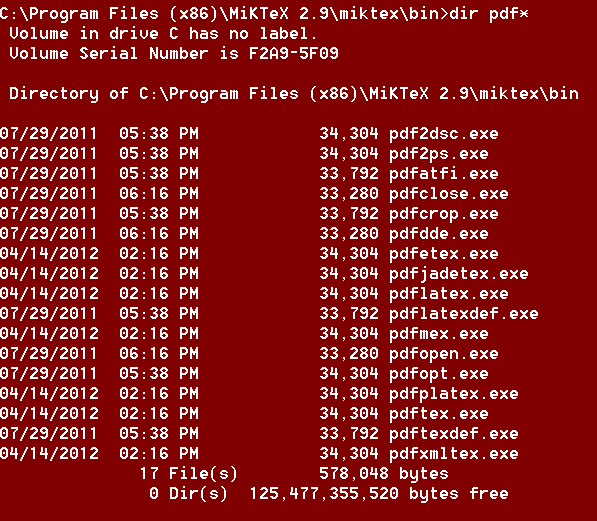
\includegraphics[width=4in]{miktex.png}
\end{figure}

\begin{figure}
\caption{Using \texttt{pdflatex.exe}}
\label{simple}
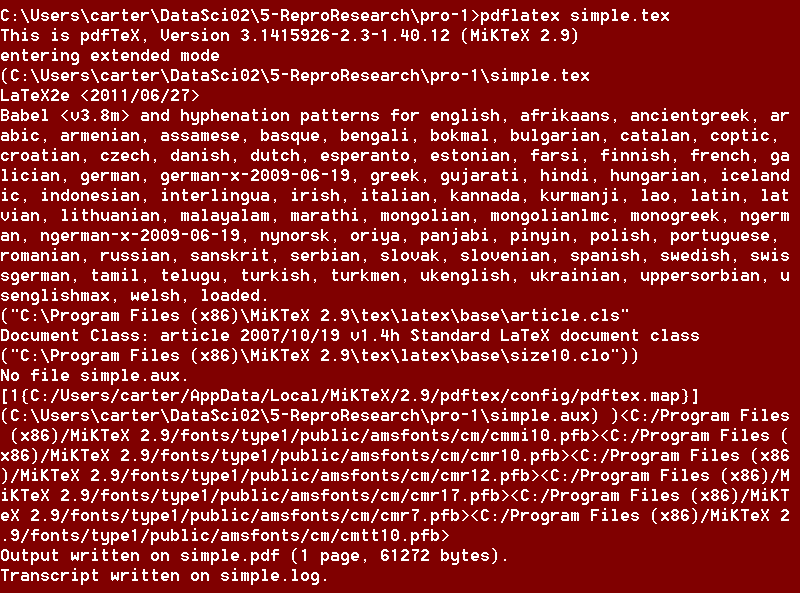
\includegraphics[width=4in]{simple.png}
\end{figure}

\section{Getting \texttt{knitr}}

\paragraph{}Invoke the \textsf{R} GUI, install the \texttt{knitr} package if you have not already done so, and load the \texttt{knitr} library. See listing \ref{load}.

\begin{lstlisting}[caption={Loading \texttt{knitr}}, label=load]
install.packages{knitr}
library{knitr}
\end{lstlisting}

\section{Creating PDF from .Rnw files}

\paragraph{}Creating a PDF document with \texttt{knitr} requires three steps: first, create a \texttt{.Rnw} source file, second, knit the source file with \texttt{knit()}, and third, compile the resulting \texttt{.tex} file with \texttt{pdflatex}. This tutorial includes a simple source file (see listing \ref{first}) named \texttt{first.Rnw}. The \textsf{R} code shamelessly cribbed from Yihui Xie at \url{http://yihui.name/knitr/}.

\begin{lstlisting}[caption={First Rnw file}, label=first]
\documentclass{article}
\title{My First Rnw File}
\author{My Name}
\date{}
\begin{document}
\maketitle{}
\paragraph{}This is my first .Rnw file, from \textsf{R} to PDF through \LaTeXe{}. 

<<my-label, eval=TRUE, dev='png'>>=
set.seed(1213)  # for reproducibility
x = cumsum(rnorm(100))
mean(x)  # mean of x
plot(x, type = 'l')  # Brownian motion
@

\end{lstlisting}

\paragraph{}In the \textsf{R} GUI, knit the \texttt{first.Rnw} source file. See figure \ref{knitting}. This will create a file named \texttt{first.tex}. Then, run \texttt{pdflatex} against this file. This will produce a PDF document names \texttt{first.pdf} that looks like figure \ref{PDF}.

\begin{figure}
\caption{Knitting}
\label{knitting}
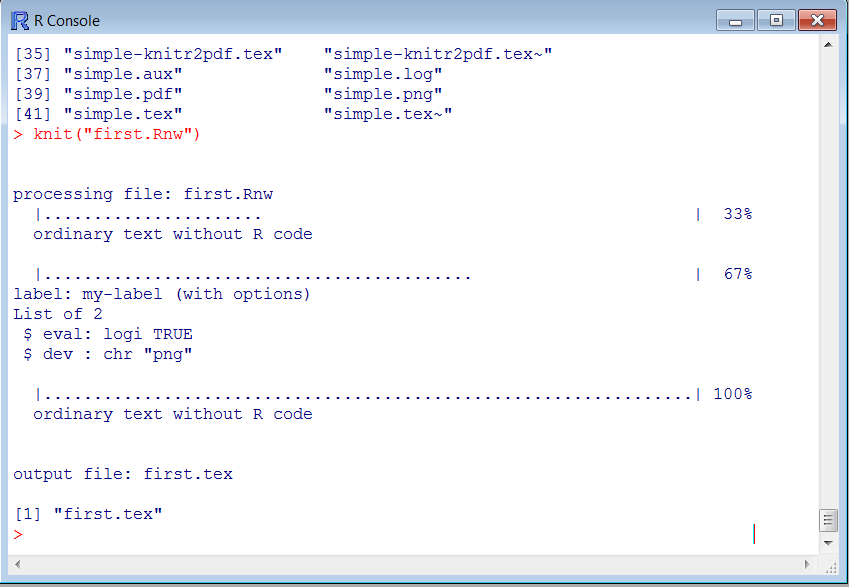
\includegraphics[width=4in]{knitting.png}
\end{figure}

\begin{figure}
\caption{first.pdf}
\label{PDF}
\fbox{\includegraphics[scale=0.5]{first.pdf}}
\end{figure}


%\begin{figure}
%\caption{first.pdf}
%\label{PDF}
%\includepdf[pages=1-2,scale=0.33]{first.pdf}
%\end{figure}



\end{document}
